\section{Introduction}\label{sec:introduction}
This chapter shows screenshots of the system interface and details the programming environment , data manipulation and programming languages used in the development of the system.

\subsection{Implementing the system}

\subsubsection{Programming Tools}
The system was implemented using the following programming tools:
\begin{itemize}
    \item \textbf{Android Studio}: This is the official IDE for Android development. It is used in the development of the mobile application.
    \item \textbf{Arduino IDE}: This is the official IDE for Arduino development. It is used in the development of the microcontroller code.
    \item \textbf{Digital Ocean}: This is a cloud hosting service. It is used to host the remote server.
    \item \textbf{Flutter}: This is a cross-platform UI toolkit developed by Google. It is used to develop the mobile application.
    \item \textbf{ESP32 Microcontroller}: This is a microcontroller developed by Espressif Systems. It is used to receive data from the mobile application and send it to the remote server.
\end{itemize}

\subsubsection{Embedded Systems Equipment}
The following equipment was used in the development of the system:
\begin{figure}[h]%
    \centering
    \subfloat[\centering]{{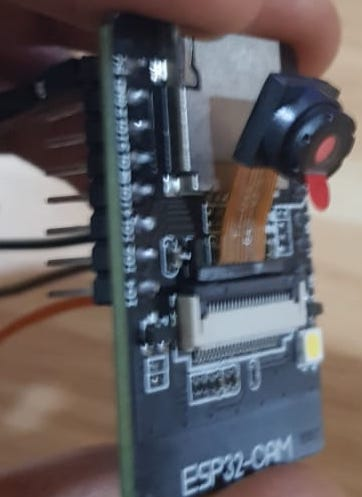
\includegraphics[scale=0.3]{images/esp1} }}%
    \qquad
    \subfloat[\centering]{{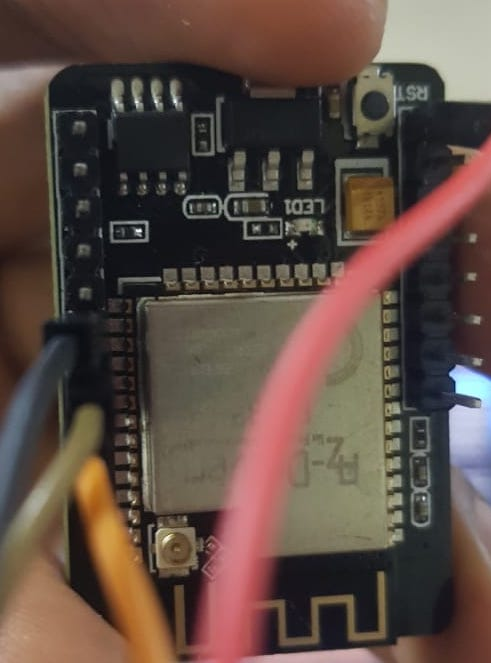
\includegraphics[scale=0.3]{images/esp2} }}%
    \caption{ESP32 microntroller used to scan the user QR codes}%
    \label{fig:equip}%
\end{figure}

\subsection{Sample Screenshots}
\begin{figure}[h]%
    \centering
    \subfloat[\centering]{{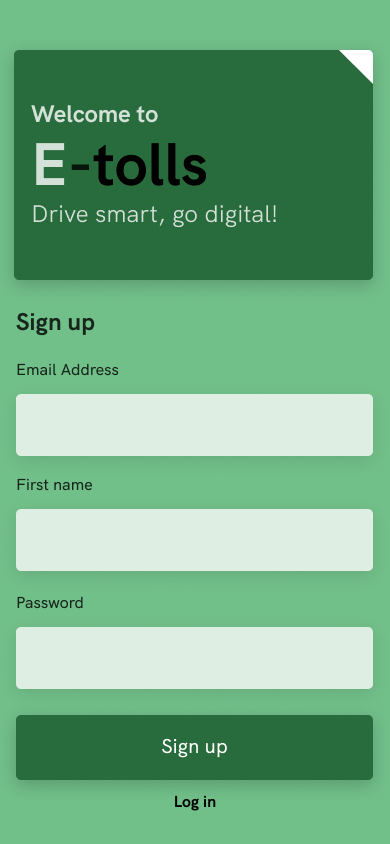
\includegraphics[scale=0.3]{images/Signup} }}%
    \qquad
    \subfloat[\centering]{{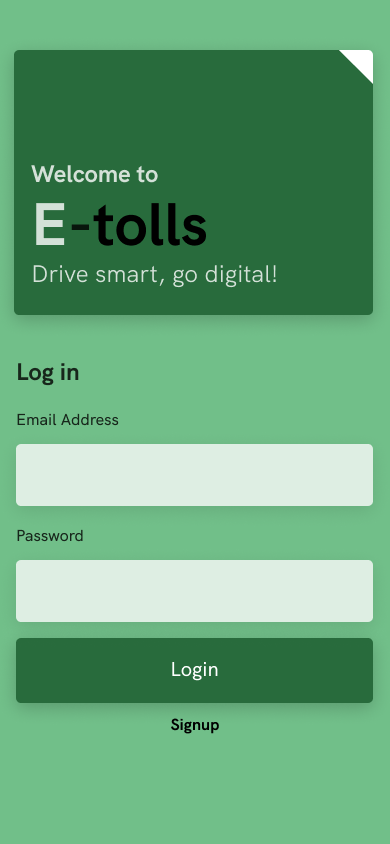
\includegraphics[scale=0.3]{images/Log in} }}%
    \caption{Login and Sign Up Screens of the mobile application}%
    \label{fig:example}%
\end{figure}

\begin{figure}[h]%
    \centering
    \subfloat[\centering]{{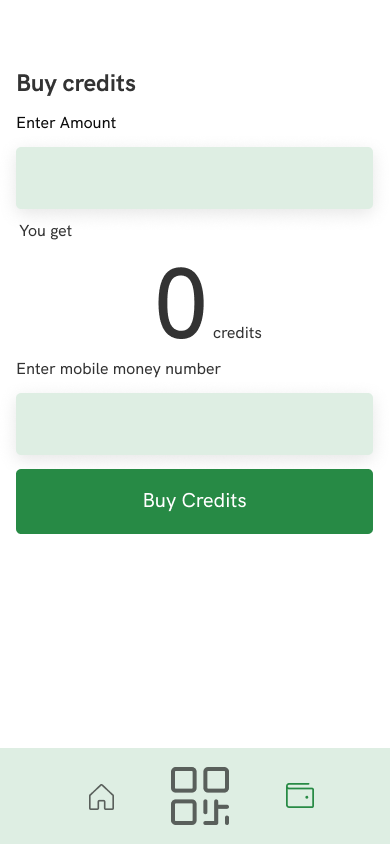
\includegraphics[scale=0.3]{images/Payments} }}%
    \qquad
    \subfloat[\centering]{{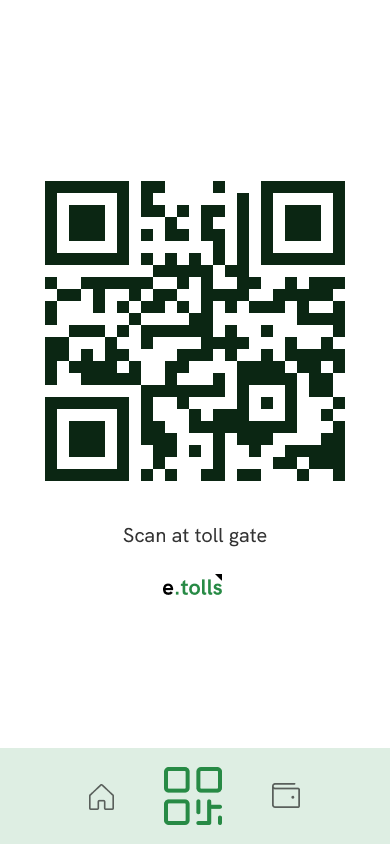
\includegraphics[scale=0.3]{images/QRCode} }}%
    \caption{Payment Screens of the mobile application}%
    \label{fig:example1}%
\end{figure}